\rhead[\thepage]{\scriptsize{CAPÍTULO \thechapter}. \rightmark}
\lhead[CAPÍTULO \thechapter. \leftmark]{}
%======================================================================
\chapter{Cálculo vectorial}
\label{CV}
\markboth{Cálculo vectorial}{Cálculo vectorial}
%======================================================================

Este capítulo tiene como objetivo comprender el cálculo vectorial, que ayuda a tener una noción mayor sobre el espacio en donde se mueven las cosas. Un vector tiene como elementos que lo describen una magnitud y una dirección. Ejemplos del uso de vectores es muy amplio sobretodo en física, por ejemplo desplazamiento, velocidad, fuerza, etc.\\

Antes de llegar a los vectores como tal se debe ver ciertos temas, para tener una base sólida al momento de enfrentarse a problemas vectoriales, uno de ellos son los ángulos y su sentido.   
%----------------------------------------------------------------------
\section{Ángulos y su orientación}
\label{CV0}
%----------------------------------------------------------------------
El ángulo se forma con dos rectas con un punto en común que se llama \textit{vértice}. Uno puede imaginar que una de las rectas queda fija (lado inicial) y la otra recta (lado terminal) rota con respecto al vértice para formar el ángulo entre las dos rectas.\\
Cuando se forma el ángulo se puede medir en grados que van desde $0$ a $360$ grados y se considera positivo cuando va en sentido antihorario, por consiguiente, si va en sentido horario la medida será negativa.

 \begin{center}
\begin{figure}[h!]
\centering
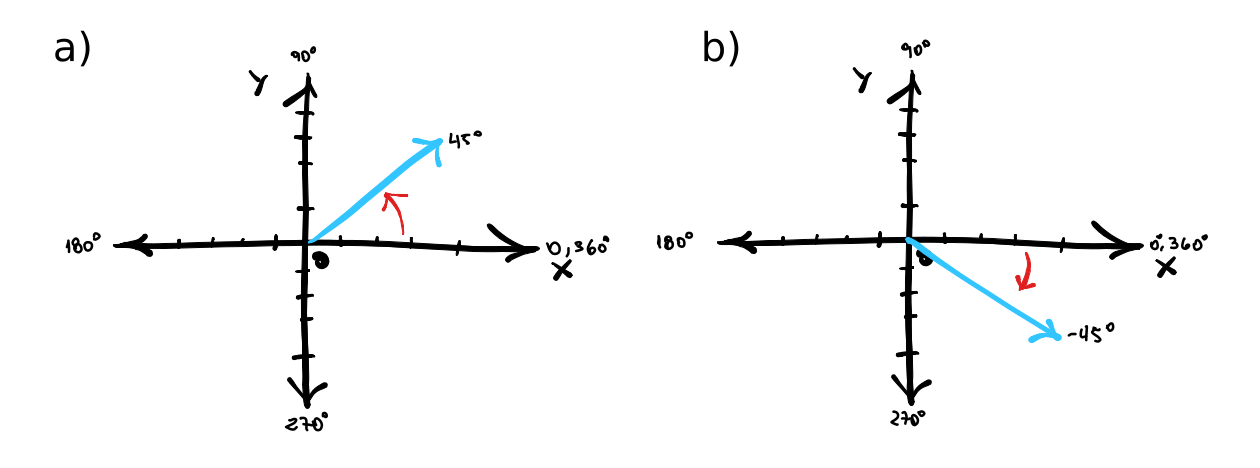
\includegraphics[scale=0.28]{ang0.png}
\caption[Figura de ángulos positivo y negativo]{Figura de ángulos positivo y negativo. a) Muestran un plano cartesiano de $x$ e $y$ donde hay un vector en $45^{o}$ en sentido positivo. b) Es un vector en el mismo plano cartesiano y también es de $45^{o}$, pero es negativo.} \label{grados0}
\end{figure}
\end{center}
Así como un ángulo se puede medir en grados, igual está la opción de medirlos en radianes. Esta unidad se basa en la longitud de un arco del un circulo centrado en el origen y de radio $1$.
\begin{eqnarray}
x^{2}+y^{2}=1
\end{eqnarray}
La convención en radianes son las mismas que en los ángulos, es decir, el sentido positivo y negativo son los mismos. Los radianes van desde $0$ a $2\pi$.

 \begin{center}
\begin{figure}[h!]
\centering
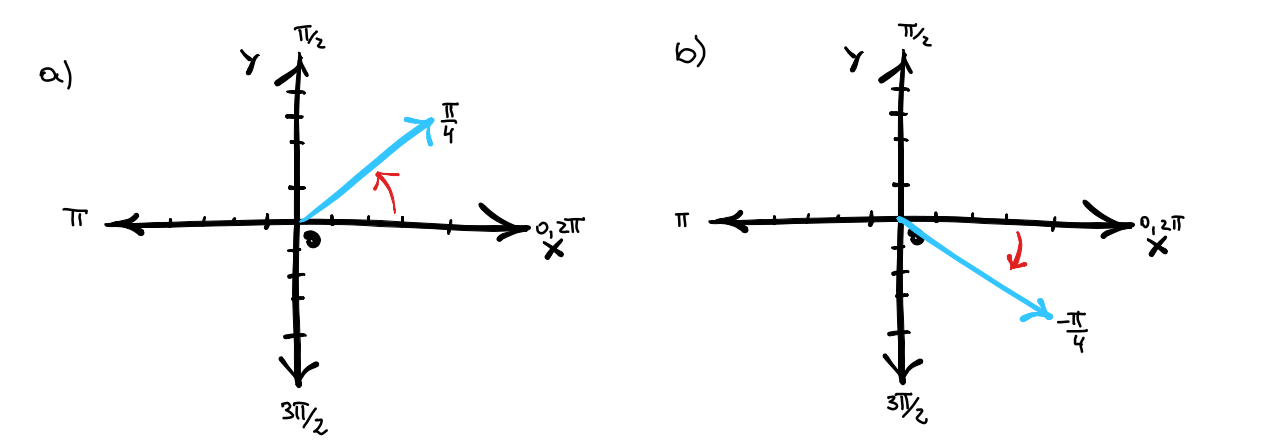
\includegraphics[scale=0.28]{ang1.png}
\caption[Figura de radianes positivo y negativo]{Figura de ángulos positivo y negativo. a) Muestran un plano cartesiano de $x$ e $y$ donde hay un vector en $\pi/4$ radianes en sentido positivo. b) Es un vector en el mismo plano cartesiano y también es de $\pi/4$ radianes, pero es negativo.} \label{grados0}
\end{figure}
\end{center}

La forma para pasar de un sistema al otro es hacer una regla de tres simples, siempre teniendo en cuenta que las equivalencias son las siguientes:
\begin{eqnarray*}
2\pi\rightarrow 360^{o}\\
x\rightarrow 45^{0}
\end{eqnarray*}
Por ejemplo, en esta regla de tres simples se quiere pasar de grados a radianes, entonces la incógnita es a cuantos radianes equivalen $45^{o}$. La respuesta es $x=\pi/4$.

El resumen de los ángulos más importantes se ven en la siguiente tabla;


\begin{table}[h!]
\begin{center}
 \begin{tabular}{|c|c|c|c|c|c|c|c|c|c|}
 \hline
 Grados $[^{o}]$ &$0$&$30$&$45$&$60$&$90$&$180$&$270$&$360$ \\
 \hline
 Radianes $[rad]$ &$0$&$\dfrac{\pi}{6}$&$\dfrac{\pi}{4}$&$\dfrac{\pi}{3}$&$\dfrac{\pi}{2}$&$\pi$&$\dfrac{3\pi}{2}$&$2\pi$ \\
 \hline
 \end{tabular}
 \caption{Tabla resumen de los ángulos más comunes en grados y su equivalente en radianes.}
 \end{center}
\end{table}

\section{Trigonometría}

Utilizaremos los ángulos mostrados en la sección anterior en funciones trigonométricas, que se pueden calcular en base a los lados de un triángulo rectángulo.\\
El triángulo rectángulo consta de 3 lados etiquetados con las letras $a$, $b$ y $c$. Además, se etiqueta un ángulo con la letra griega \textit{theta} $\theta$. El lado opuesto al ángulo recto se llama hipotenusa, el cateto que se une en un vértice con la hipotenusa y además contiene el ángulo $\theta$ se llama cateto adyacente y el cateto que no contiene al ángulo $\theta$ es el cateto opuesto.

\begin{center}
\begin{figure}[h!]
\centering
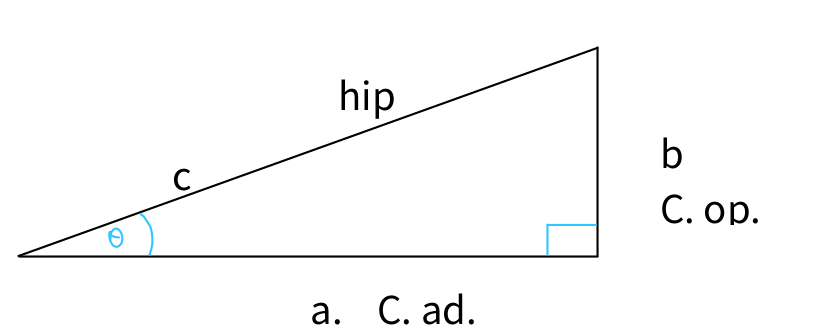
\includegraphics[scale=0.30]{trig0.png}
\caption[Triangulo rectángulo con las etiquetas sus catetos e hipotenusa]{Triángulo rectángulo con las etiquetas sus catetos e hipotenusa. El lado a es el cateto adyacente, b es el cateto opuesto y c es la hipotenusa. El ángulo entre el cateto adyacente y la hipotenusa se etiqueta con $\theta$. } \label{trig0}
\end{figure}
\end{center}

\begin{mydef}
\textbf{Funciones trigonométricas. }En base al triangulo de la figura (\ref{trig0}) se definen las siguientes funciones trigonométricas:
\begin{eqnarray}
sen(\theta)&=&\dfrac{C. op.}{hip}\\
cos(\theta)&=&\dfrac{C. ad.}{hip}\\
tan(\theta)&=&\dfrac{C. op}{C. ad}=\dfrac{sen(\theta)}{cos(\theta)}\\
cot(\theta)&=&\dfrac{C. ad}{C. op}=\dfrac{1}{tan(\theta)}\\
sec(\theta)&=&\dfrac{hip}{C. ad.}=\dfrac{1}{cos(\theta)}\\
csc(\theta)&=&\dfrac{hip}{C. op}=\dfrac{1}{sen(\theta)}
\end{eqnarray}
Las abreviaciones son las siguientes: sen=seno, cos=coseno, tan=tangente, cot=cotangente, sec=secante y csc=cosecante.
\end{mydef}

El triángulo de la figura (\ref{trig0}) al ser rectángulo cumple el teorema de Pitágoras, entonces se puede usar para formular las soguientes identidades trigonométricas. 
\begin{eqnarray}
a^{2}+b^{2}=c^{c}
\label{pitagoras}
\end{eqnarray} 
Si (\ref{pitagoras}) lo dividimos por $a^{2}$, $b^{2}$ y $c^{c}$ se obtienen las siguientes ecuaciones.\\

\noindent a) Dividir por $c^{2}:$
\begin{eqnarray}
a^{2}+b^{2}=c^{c} \\
\left(\dfrac{a}{c}\right)^{2}+\left(\dfrac{b}{c}\right)^{2}=1
\end{eqnarray}

\noindent a) Dividir por $b^{2}:$
\begin{eqnarray}
a^{2}+b^{2}=c^{c} \\
\left(\dfrac{a}{b}\right)^{2}+1=\left(\dfrac{c}{b}\right)^{2}
\end{eqnarray}

\noindent a) Dividir por $a^{2}:$
\begin{eqnarray}
a^{2}+b^{2}=c^{c} \\
1+\left(\dfrac{b}{a}\right)^{2}=\left(\dfrac{c}{a}\right)^{2}
\end{eqnarray}
Si las ecuaciones anteriores lo pasamos a funciones trigonométricas se forman las siguientes identidades

\begin{mydef}
\textbf{Identidades trigonométricas. }
\begin{eqnarray}
sen^{2}(\theta)+cos^{2}(\theta)=1\\
1+tan^{2}(\theta)=sec^{2}(\theta)\\
cot^{2}(\theta)+1=csc^{2}(\theta)
\end{eqnarray}
\end{mydef}

Si se junta las funciones trigonométricas con lo visto de los ángulos en grados y radianes se puede resumir en una tabla con los valores más comunes.

\begin{table}[h!]
\begin{center}
 \begin{tabular}{|c|c|c|c|c|c|c|c|}
 \hline
Grados &$0^{o}$&$30^{o}=\pi/6$&$45^{o}=\pi/4$&$60^{o}=\pi/3$&$90^{o}=\pi/2$&$270^{o}=3\pi/2$ \\
 \hline
 $sen(\theta)$&$0$&$\dfrac{1}{2}$&$\dfrac{\sqrt{2}}{2}$&$\dfrac{\sqrt{3}}{2}$&$1$&$-1$ \\
 \hline
 $cos(\theta)$&$1$&$\dfrac{\sqrt{3}}{2}$&$\dfrac{\sqrt{2}}{2}$&$\dfrac{1}{2}$&$0$&$0$ \\
 \hline
 $tan(\theta)$&$0$&$\dfrac{\sqrt{3}}{3}$&$1$&$\sqrt{3}$&$\infty$&$\infty$ \\
 \hline
 \end{tabular}
 \caption{Tabla resumen de los valores mas comunes de las funciones trigonométricas.}
 \end{center}
\end{table}

\begin{myexample}
Encuentre el valor de la siguiente expresión:
\begin{eqnarray*}
cos(30^{o})\cdot tan(60^{o})=\dfrac{\sqrt{3}}{2}\cdot\sqrt{3}=\dfrac{3}{2}
\end{eqnarray*}
\end{myexample}

\section{Vectores}

Cuando uno se enfrenta a los problemas de mover cosas o desplazarse, uno hace un mapa o plano mental de como moverse y de forma inconsciente hacemos las direcciones. Si se plasma ese plano mental, naturalmente lo llevaremos a \textit{flechas} que nos direccionan a nuestro destino. Estas flechas con un largo y dirección lo llamaremos \textit{vector}.\\

Gráficamente, el vector es representado por una flecha entre dos puntos, donde tiene un punto inicial y final que define su dirección. Si los puntos que son $O$ y $P$ el trazo $OP$ forma el vector denotado por $\vec{A}$ y el largo del vector se llama magnitud y es denotado $|\vec{A}|$.\\

 \begin{center}
\begin{figure}[h!]
\centering
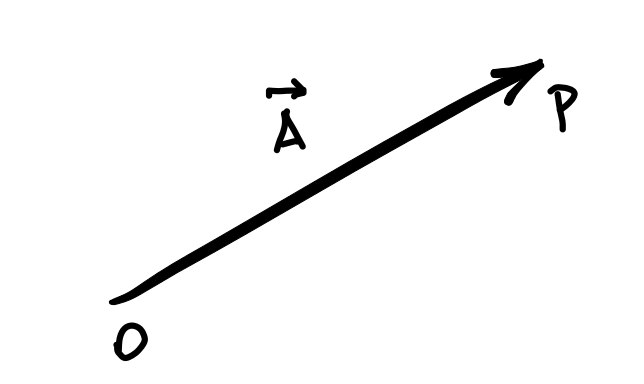
\includegraphics[scale=0.30]{vect0.png}
\caption[Representación de un vector.]{Representación de un vector. El punto inicial es el $O$, el punto final es el $P$ y el largo es la magnitud.} \label{vect0}
\end{figure}
\end{center}

La magnitud es un número y no tiene dirección, a estas cantidades se les llama \textit{escalares}. Ejemplos de magnitudes escalares son: La masa, largo, tiempo, temperatura y cualquier cantidad que sea un número real.

\begin{eqnarray}
\vec{A}=|\vec{A}|\cdot\vec{e}
\label{vector0}
\end{eqnarray}
El vector $\vec{A}$ cuenta con un número escalar que es la magnitud y un vector que le da la dirección. Un ejemplo que sirve por el momento es decir que uno se puede mover $10m$, pero es distinto decir que uno se moverá $10m$ al sur o al norte. El decir norte o sur da la dirección a la cual uno se desplazará.
\begin{itemize}
	\item Sea $\vec{A}$ y $\vec{B}$ dos vectores y se dicen que son iguales si tienen la misma magnitud y dirección sin importar sus puntos de inicio. Ver representación a) de la figura (\ref{vect1}).\\
	\item Un vector $\vec{A}$, pero con dirección opuesta y misma magnitud se denota como $-\vec{A}$. Ver representación b) de la figura (\ref{vect1}).
\end{itemize}

 \begin{center}
\begin{figure}[h!]
\centering
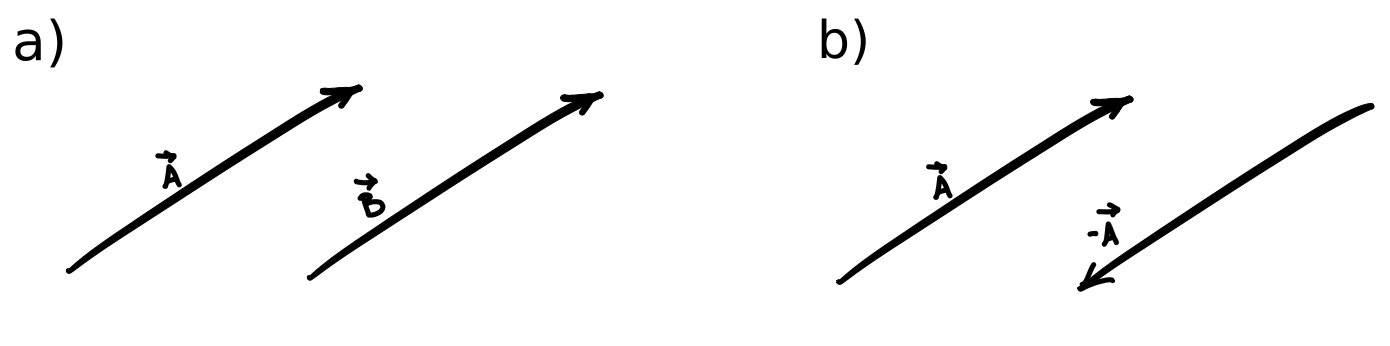
\includegraphics[scale=0.25]{vect1.png}
\caption[Representación 
Representación de vectores iguales y opuestos.]{Representación de vectores iguales y opuestos. a) Se muestran dos vectores iguales que son iguales en magnitud y sentido. b) Se muestran dos vectores opuestos que son iguales en magnitud pero distintos en sentido.} \label{vect1}
\end{figure}
\end{center}

Las operaciones posibles con los vectores son la suma, la resta y la multiplicación. Por parte de la suma de dos vectores se forma un vector resultante donde el inicio calza con el inicio del primer vector y termina con el punto final del segundo vector. En la resta se une ambos puntos finales de los vectores (ver figura \ref{vect2}).

 \begin{center}
\begin{figure}[h!]
\centering
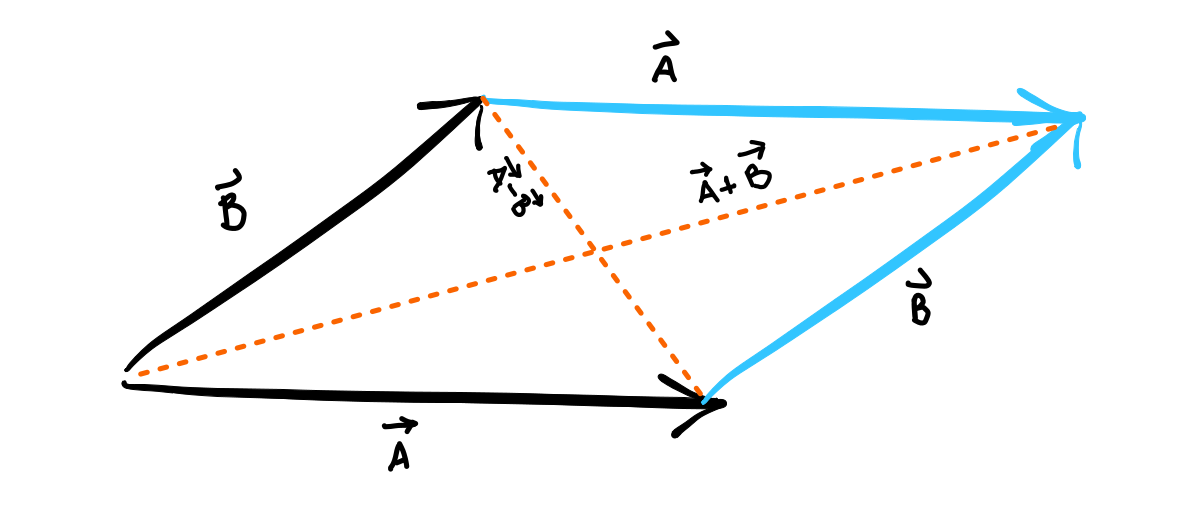
\includegraphics[scale=0.25]{vect2.png}
\caption[Representación de la suma y resta de dos vectores.]{Representación de la suma y resta de dos vectores. Se muestran los vectores $\vec{A}$ y $\vec{B}$ donde son duplicados para mostrar como es el vector resultante de la suma y la resta de ellos mismo.} \label{vect2}
\end{figure}
\end{center}

En términos matemáticos, cuando se aplica la operación de suma o resta se debe aplicar en cada un de los elementos. La primera forma de ver un vector en más de una dimensión es un paréntesis donde cada número representa la magnitud que tiene en cada dirección. Entonces, considere dos vectores $\vec{v}_{1}=(x_{1},y_{1},z_{1})$ y $\vec{v}_{2}=(x_{2},y_{2},z_{2})$ donde la suma y la resta queda definida como:\\

\noindent a) Suma:\\
\begin{eqnarray}
\vec{v}_{1}+\vec{v}_{2}&=&(x_{1},y_{1},z_{1})+(x_{2},y_{2},z_{2})\\
&=&(x_{1}+x_{2},y_{1}+y_{2},z_{1}+z_{2})
\end{eqnarray}
\noindent a) Resta:\\
\begin{eqnarray}
\vec{v}_{1}-\vec{v}_{2}&=&(x_{1},y_{1},z_{1})-(x_{2},y_{2},z_{2})\\
&=&(x_{1}-x_{2},y_{1}-y_{2},z_{1}-z_{2})
\end{eqnarray}

\begin{mydef}
\textbf{Algebra de los vectores. }Si $\vec{A}$, $\vec{B}$ y $\vec{C}$ son vectores y $m$ y $n$ son escalares, entonces se cumple las siguientes leyes:
\end{mydef}
\begin{eqnarray}
\vec{A}+\vec{B}&=&\vec{B}+\vec{A}\\
\vec{A}+(\vec{B}+\vec{C})&=&(\vec{A}+\vec{B})+\vec{C}\\
m\vec{A}&=&\vec{A}m\\
m(n\vec{A})&=&(mn)\vec{A}\\
(m+n)\vec{A}&=&m\vec{A}+n\vec{A}\\
m(\vec{A}+\vec{B})&=&m\vec{A}+m\vec{B}
\end{eqnarray}



\subsection{Vectores unitarios}

En la ecuación (\ref{vector0}) presentamos a $\vec{e}$ que nos dice la dirección del vector. Este elemento se le llama vector unitarios, es decir, tiene largo uno.\\
Cuando creamos un plano en 2D o un espacio en 3D para colocar los vectores, cada eje tiene un vector unitario. A diferencia de cualquier vector, la notación de un vector unitario es $\hat{i}, \hat{j}$ y $\hat{k}$.

 \begin{center}
\begin{figure}[h!]
\centering
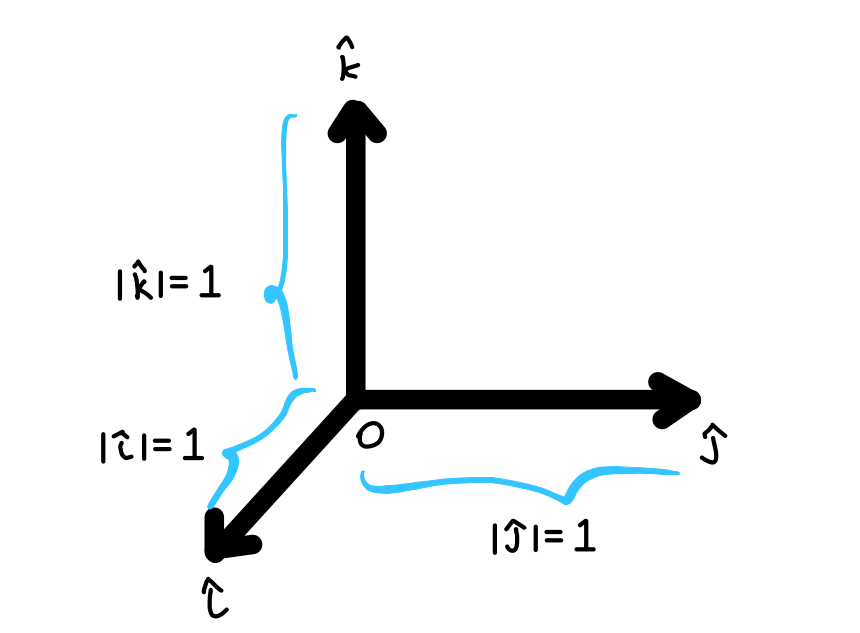
\includegraphics[scale=0.25]{vect3.png}
\caption[Representación de los vectores unitarios.]{Representación de los vectores unitarios. Se muestra que el largo de cada uno de los vectores es 1 partiendo desde el origen.} \label{vect3}
\end{figure}
\end{center}

\begin{myexample}
Sea $\vec{A}=5\hat{i}$, calcule el doble del vector $\vec{A}$.
\begin{eqnarray*}
\vec{A}&=&5\hat{i}\\
2\cdot\vec{A}&=&2\cdot 5\hat{i}\\
2\cdot\vec{A}&=&10\hat{i}\\
\end{eqnarray*}
\end{myexample}

Ahora cualquier vector se puede  volver un vector unitario. Si un vector $\vec{A}$ tiene una norma distinta de uno, se debe dividir por un escalar y es su propia magnitud.
\begin{eqnarray}
\vec{A}=\dfrac{\vec{A}}{|\vec{A}|}
\end{eqnarray}

\subsection{Componentes de un vector}

Así como en un principio se dijo que era importante decir la dirección del vector, si era sur o norte, pero que ocurre si la dirección es Noroeste. El vector tiene una parte hacia el norte y una parte hacia el oeste. En estos vectores se dice que tiene componentes en esas direcciones. Si generalizamos con los ejes que hemos planteado un vector puede tener componentes en los ejes $\hat{i}, \hat{j}$ y $\hat{k}$. Esto se puede extender a cuantas componentes nosotros queramos, pero para este curso veremos el caso de dos y tres dimensiones.
\begin{eqnarray}
\vec{A}=A_{1}\hat{i}+A_{2}\hat{j}+A_{3}\hat{k}
\label{vector1}
\end{eqnarray}
Lo importante de (\ref{vector1}) es que nos permite calcular la magnitud de un vector cualquiera en base a sus componentes.\\

 \begin{center}
\begin{figure}[h!]
\centering
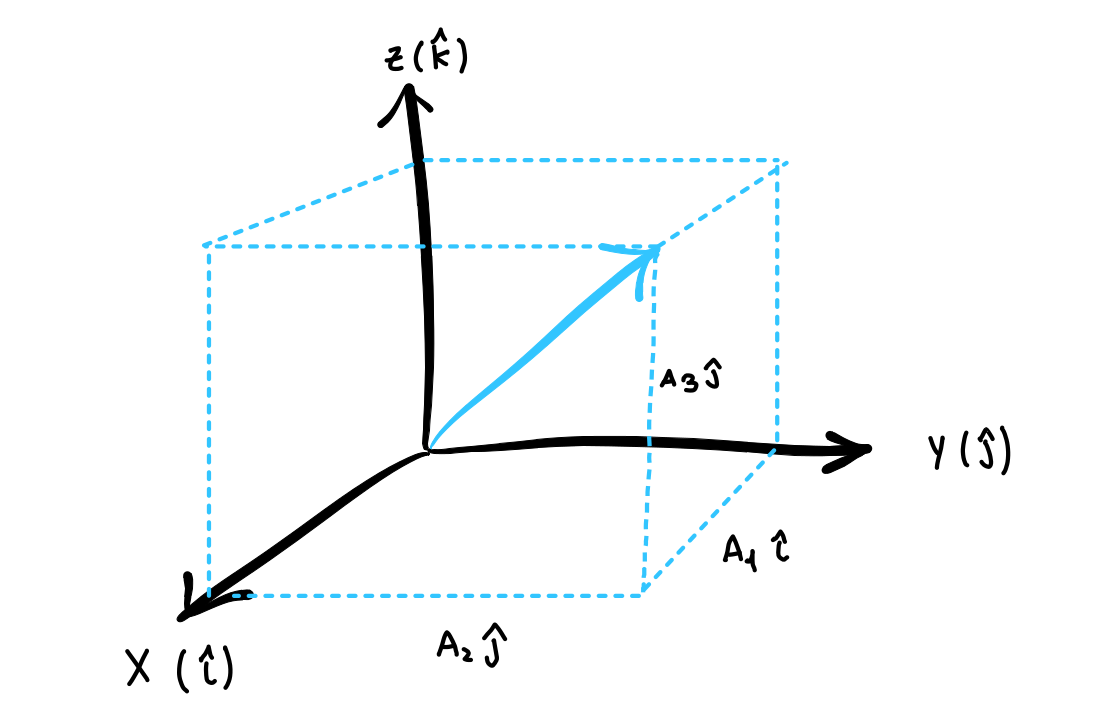
\includegraphics[scale=0.25]{vect4.png}
\caption[Representación de las componentes de un vector.]{Representación de las componentes de un vector en tres dimensiones. El vector muestra componente los tres ejes etiquetados como $A_{1}$ en el eje $x$, $A_{2}$ en el eje $y$ y $A_{3}$ en el eje $z$.} \label{vect4}
\end{figure}
\end{center}


 Si suponemos que tenemos un vector llamado $\vec{r}$ con componentes $(x,$ $y$, $z)$ y queremos calcular su magnitud debemos hacer lo siguiente
\begin{eqnarray*}
\vec{r}&=&x\vec{i}+y\vec{j}+z\vec{k}\\
|\vec{r}|&=&\sqrt{x^{2}+y^{2}+z^{2}}
\end{eqnarray*} 

\begin{myexample}
Sea $\vec{v}=3\hat{i}+4\hat{j}+5\hat{k}$. Calcule la magnitud del vector $\vec{v}$
\begin{eqnarray*}
\vec{v}&=&3\hat{i}+4\hat{j}+5\hat{k}\\
|\vec{v}|&=&\sqrt{3^{2}+4^{2}+5^{2}}\\
|\vec{v}|&=&\sqrt{9+16+25}\\
|\vec{v}|&=&\sqrt{50}\\
|\vec{v}|&=&\sqrt{25\cdot 2}\\
|\vec{v}|&=&\sqrt{25}\cdot \sqrt{2}\\
|\vec{v}|&=&5\sqrt{2}\\
\end{eqnarray*}
\end{myexample}

\begin{myexample}
Sea $\vec{v}=3\hat{i}+4\hat{j}+5\hat{k}$. ormalice del vector $\vec{v}$:
\begin{eqnarray*}
\vec{v}&=&3\hat{i}+4\hat{j}+5\hat{k}\\
\hat{v}&=&\dfrac{\vec{v}}{|\vec{v}|}\\
\hat{v}&=&\dfrac{1}{5\sqrt{2}}\left( 3\hat{i}+4\hat{j}+5\hat{k}\right)\\
\end{eqnarray*}
Norma de $|\hat{v}|$
\begin{eqnarray*}
|\hat{v}|&=&\sqrt{\left(\dfrac{3}{5\sqrt{2}}\right)^{2}+\left(\dfrac{4}{5\sqrt{2}}\right)^{2}+\left(\dfrac{5}{5\sqrt{2}}\right)^{2}}\\
&=&\sqrt{\left(\dfrac{9}{25\cdot 2}\right)+\left(\dfrac{16}{25\cdot 2}\right)+\left(\dfrac{25}{25\cdot 2}\right)}\\
&=&\sqrt{\left(\dfrac{9}{50}\right)+\left(\dfrac{16}{50}\right)+\left(\dfrac{25}{50}\right)}\\
&=&\sqrt{\left(\dfrac{9+16+25}{50}\right)}\\
&=&\sqrt{\left(\dfrac{50}{50}\right)}\\
&=&\sqrt{\left(1\right)}\\
|\hat{v}|&=&1\\
\end{eqnarray*}
\end{myexample}



